\documentclass[aps,prd,twocolumn,10pt,nofootinbib]{revtex4-2}
% Fallback if revtex is unavailable: \documentclass[twocolumn,10pt]{article} + \usepackage{amsmath,amssymb}
\usepackage{amsmath,amssymb,graphicx}
\usepackage{pgfplots}
\pgfplotsset{compat=1.16}
\usepackage[colorlinks=true,linkcolor=blue,citecolor=blue]{hyperref}

\begin{document}

\title{One Law for the Radial Acceleration Relation and the External Field Effect:\\
the de Sitter--Unruh Interpolation and $a_0=c^2\sqrt{\Lambda/32\pi}$}
\author{C.\ Zimmerman}
\date{June 2026}

\begin{abstract}
The \emph{external field effect} (EFE) is the sharpest qualitative test separating modified gravity from particle
dark matter: a uniform external field cannot touch a system's internal dynamics under Newton$+$dark matter, but
\emph{must} in any non-linear modified-gravity law. This paper is the internally-consistent companion to an
earlier treatment: there the isolated radial acceleration relation (RAR) used the framework's de Sitter--Unruh
interpolation $g_{\rm obs}=\sqrt{g_{\rm bar}^2+g_{\rm bar}a_0}$ while the EFE was written with the unrelated
``simple'' MOND interpolation $\nu=\tfrac12+\sqrt{\tfrac14+1/y}$. A modified-gravity theory has \emph{one}
interpolation function; here we use the framework's own de Sitter--Unruh form $\nu(y)=\sqrt{1+1/y}$ for
\emph{both} the RAR and the EFE, at the framework's own acceleration scale $a_0=c^2\sqrt{\Lambda/32\pi}=
9.36\times10^{-11}\,\mathrm{m\,s^{-2}}$. The qualitative physics is unchanged; the quantitative predictions
sharpen and, honestly, \emph{shrink}: because $a_0$ is lower than the canonical MOND value, the Milky Way's
external field sits at $g_{\rm ext}=2.30\,a_0$ (not $1.8\,a_0$), driving the system deeper into the
external-field-suppressed regime. The wide-binary boost is $G_{\rm eff}/G\simeq1.14$ (orbit-averaged;
$+6.6\%$ in velocity), \emph{not} the $1.3$ of the simple interpolation. We give the corrected figures, state the
current data placement honestly (consistent with, but not confirmed against, present wide-binary measurements),
and keep the acceleration scale's coefficient an explicit, underived posit.
\end{abstract}

\maketitle

\section{Two explanations, one decisive test}
Spiral galaxies rotate too fast for their visible mass: below a characteristic acceleration the observed
acceleration $g_{\rm obs}$ exceeds the Newtonian value $g_{\rm bar}$ from baryons alone, following the tight
\emph{radial acceleration relation} (RAR), with $g_{\rm obs}\!\to\!\sqrt{a_0\,g_{\rm bar}}$ at low
accelerations~\cite{McGaugh2016}. Two pictures explain this. \emph{Dark matter}: each galaxy sits in a halo of
unseen particles. \emph{Modified gravity} (MOND~\cite{Milgrom1983}): gravity itself is enhanced below $a_0$, with
no new matter. On rotation curves the two are nearly degenerate. The \emph{external field effect} breaks the
degeneracy cleanly, because it tests a \emph{principle} rather than a fit: does a system's internal gravity care
about the gravitational field of its surroundings?

\section{Why dark matter forbids it, and modified inertia requires it}
\textbf{Newton $+$ dark matter: no effect.} Newtonian gravity obeys the \emph{strong equivalence principle}: a
spatially uniform external field $\mathbf{g}_{\rm ext}$ accelerates every part of a system equally and cancels
from the internal equations of motion. A dwarf galaxy falling through a cluster has the \emph{same} internal
dynamics as one in deep space. Internal physics is blind to the external field.

\textbf{The framework: an unavoidable effect.} In this framework the modification is to \emph{inertia}, arising
from the de Sitter--Unruh temperature $T_{\rm eff}=(\hbar/2\pi c k_B)\sqrt{a^2+(cH)^2}$ a body reads off the
accelerated vacuum. The response to a force depends on the \emph{total} acceleration the body actually carries---
internal $+$ external---so a uniform $\mathbf{g}_{\rm ext}$ shifts the operating point and changes the
\emph{internal} gravity. The strong equivalence principle is violated; this is a \emph{prediction}, not a defect.
Quantitatively, the framework's isolated law is the de Sitter--Unruh interpolation
\begin{equation}
g_{\rm obs}=\sqrt{g_{\rm bar}^2+g_{\rm bar}\,a_0}\;\equiv\;\nu(g_{\rm bar})\,g_{\rm bar},
\qquad \nu(y)=\sqrt{1+\tfrac{a_0}{y}},
\label{eq:rar}
\end{equation}
with the deep-MOND limit $g_{\rm obs}\!\to\!\sqrt{a_0 g_{\rm bar}}$ and the Newtonian limit $g_{\rm obs}\!\to\!
g_{\rm bar}$. The EFE is obtained from the \emph{same} $\nu$ by the one-dimensional aligned-field construction
\begin{equation}
g_{\rm obs}=\nu(g_N{+}g_{\rm ext})\,(g_N{+}g_{\rm ext})-\nu(g_{\rm ext})\,g_{\rm ext}.
\label{eq:efe}
\end{equation}
For $g_{\rm ext}\!=\!0$ this reduces to Eq.~\eqref{eq:rar}. \emph{Using $\nu(y)=\sqrt{1+a_0/y}$ in both
Eqs.~\eqref{eq:rar} and \eqref{eq:efe}---rather than borrowing the unrelated ``simple'' interpolation
$\nu=\tfrac12+\sqrt{\tfrac14+a_0/y}$ for the EFE---is the single change that makes the theory use one law. It is
required for internal consistency: a modified-gravity/inertia theory has one interpolation, fixed by its
dynamics, not two chosen by convenience.}

\textbf{The key limit.} Deep inside a system ($g_N\!\ll\!g_{\rm ext}$) in a weak external field, expand
Eq.~\eqref{eq:efe} to first order in $g_N$:
\begin{equation}
g_{\rm obs}\simeq g_N\,\nu(g_{\rm ext})\Big[1+\tfrac{d\ln\nu}{d\ln g_{\rm ext}}\Big]\equiv g_N\,\frac{G_{\rm
eff}}{G},
\label{eq:geff}
\end{equation}
with, for the de Sitter--Unruh $\nu$, the closed form $d\ln\nu/d\ln g_{\rm ext}=-\tfrac12\,[\,1+g_{\rm
ext}/a_0\,]^{-1}$. The internal dynamics are Newtonian but with a constant $G_{\rm eff}$ set by the
\emph{external} field alone. As $g_{\rm ext}\!\to\!0$ the full boost returns; as $g_{\rm ext}\!\gg\!a_0$,
$G_{\rm eff}\!\to\!G$ and gravity becomes exactly Newtonian. The external field \emph{erases} the boost.

\section{The prediction, in pictures}
Figure~\ref{fig:rar} plots the RAR from Eq.~\eqref{eq:efe} on the framework's de Sitter--Unruh $\nu$ for an
isolated galaxy and for environmental fields of $0.05\,a_0$, $0.2\,a_0$, and $1.0\,a_0$. The isolated curve
(blue) follows the deep-MOND slope $\tfrac12$; a galaxy in an external field bends to a \emph{plateau} parallel
to Newton once $g_N\!<\!g_{\rm ext}$, raised by $\nu(g_{\rm ext})$ and lowered as the field strengthens. This
environment-dependent flattening is the EFE's signature and is impossible for Newton$+$dark matter.

\begin{figure}[t]
\centering
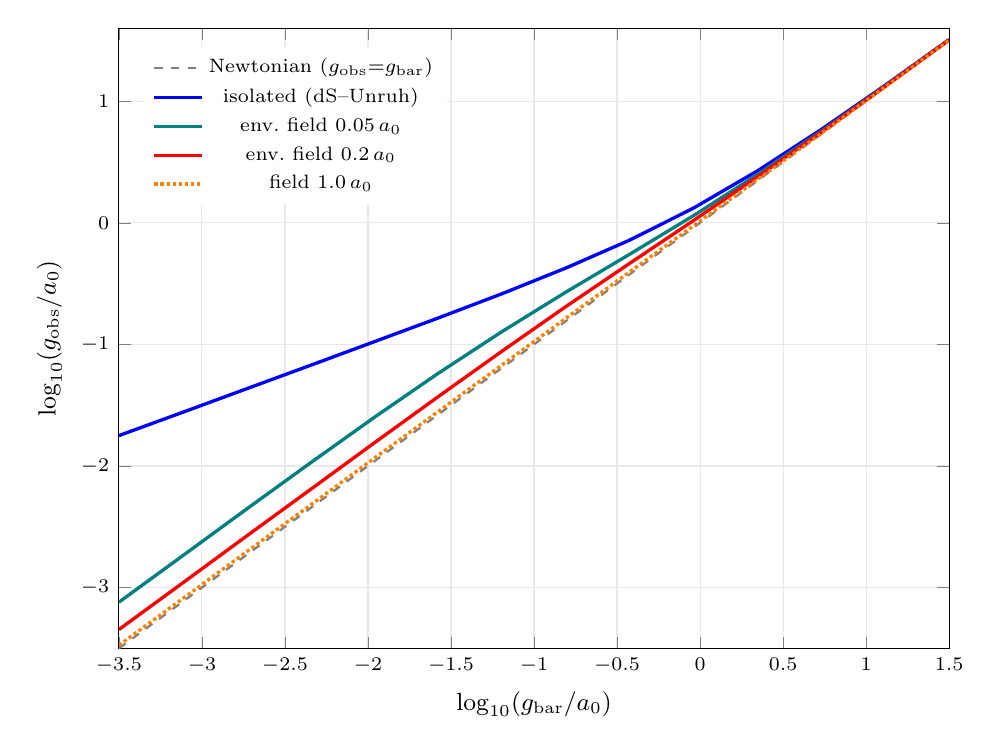
\begin{tikzpicture}
\begin{axis}[width=\columnwidth,height=0.78\columnwidth,
  xlabel={$\log_{10}(g_{\rm bar}/a_0)$}, ylabel={$\log_{10}(g_{\rm obs}/a_0)$},
  legend pos=north west, legend style={font=\scriptsize,draw=none},
  grid=both, grid style={gray!18}, xmin=-3.5, xmax=1.5, ymin=-3.5, ymax=1.6,
  tick label style={font=\scriptsize}, label style={font=\small}]
\addplot[dashed,gray,thick,domain=-3.5:1.5,samples=2]{x}; \addlegendentry{Newtonian ($g_{\rm obs}{=}g_{\rm bar}$)}
\addplot[blue,very thick] coordinates {(-3.500,-1.750)(-3.115,-1.558)(-2.731,-1.365)(-2.346,-1.172)(-1.962,-0.978)(-1.577,-0.783)(-1.192,-0.583)(-0.808,-0.372)(-0.423,-0.142)(-0.038,0.122)(0.346,0.427)(0.731,0.768)(1.115,1.131)(1.500,1.507)};
\addlegendentry{isolated (dS--Unruh)}
\addplot[teal,very thick] coordinates {(-3.500,-3.120)(-3.115,-2.737)(-2.731,-2.354)(-2.346,-1.974)(-1.962,-1.600)(-1.577,-1.238)(-1.192,-0.894)(-0.808,-0.570)(-0.423,-0.258)(-0.038,0.060)(0.346,0.397)(0.731,0.754)(1.115,1.126)(1.500,1.504)};
\addlegendentry{env.\ field $0.05\,a_0$}
\addplot[red,very thick] coordinates {(-3.500,-3.345)(-3.115,-2.961)(-2.731,-2.576)(-2.346,-2.193)(-1.962,-1.810)(-1.577,-1.430)(-1.192,-1.055)(-0.808,-0.689)(-0.423,-0.333)(-0.038,0.020)(0.346,0.378)(0.731,0.746)(1.115,1.122)(1.500,1.503)};
\addlegendentry{env.\ field $0.2\,a_0$}
\addplot[orange,very thick,densely dotted] coordinates {(-3.500,-3.474)(-3.115,-3.090)(-2.731,-2.705)(-2.346,-2.321)(-1.962,-1.936)(-1.577,-1.552)(-1.192,-1.168)(-0.808,-0.785)(-0.423,-0.403)(-0.038,-0.023)(0.346,0.356)(0.731,0.736)(1.115,1.118)(1.500,1.501)};
\addlegendentry{field $1.0\,a_0$}
\end{axis}
\end{tikzpicture}
\caption{The radial acceleration relation with the external field effect, on the framework's de Sitter--Unruh
interpolation used for \emph{both} the isolated RAR and the EFE. An isolated galaxy (blue) lifts along the
deep-MOND slope $\tfrac12$; a galaxy in an environmental field bends to a plateau parallel to Newton, raised by
$\nu(g_{\rm ext})$ and lowered as the field strengthens. The dependence on the \emph{environment} is forbidden
for Newton$+$dark matter.}
\label{fig:rar}
\end{figure}

Figure~\ref{fig:boost} isolates the magnitude: the boost $g_{\rm obs}/g_{\rm bar}$ deep in the MOND regime
($g_{\rm bar}=0.01\,a_0$) as a function of the external field. With no external field the boost is $\sim\!10$;
a Milky-Way-like field, which on the framework's $a_0$ sits at $g_{\rm ext}=2.30\,a_0$, cuts it to $\approx1.0$
along the field axis. The orbit-averaged boost for a wide binary in that field is $G_{\rm eff}/G\simeq1.14$
($+6.6\%$ in velocity)---between zero (dark matter) and the isolated value, and \emph{smaller} than the $\sim1.3$
of the simple interpolation precisely because the lower $a_0$ deepens the suppression.

\begin{figure}[t]
\centering
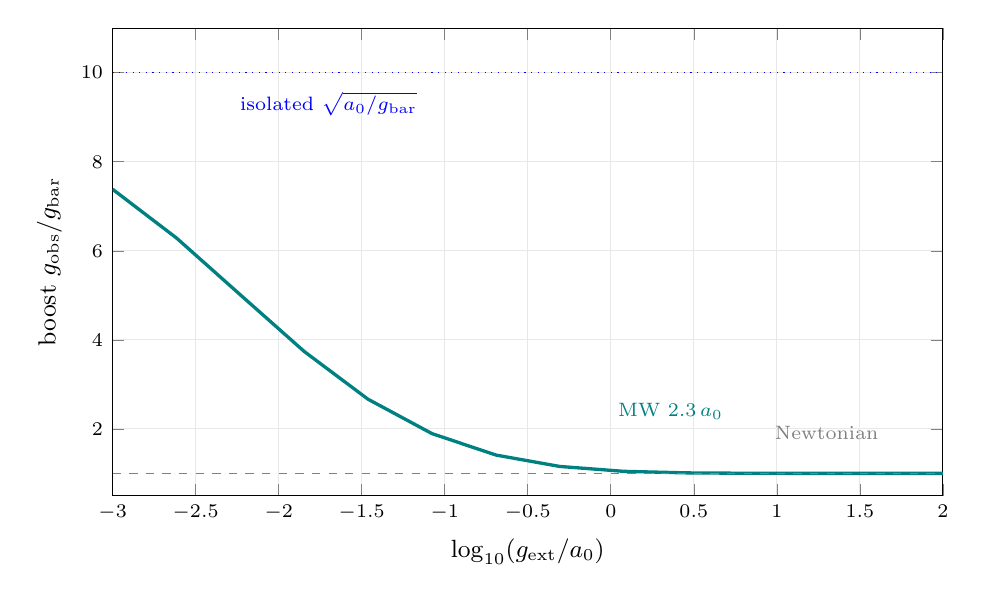
\begin{tikzpicture}
\begin{axis}[width=\columnwidth,height=0.62\columnwidth,
  xlabel={$\log_{10}(g_{\rm ext}/a_0)$}, ylabel={boost $g_{\rm obs}/g_{\rm bar}$},
  grid=both, grid style={gray!18}, xmin=-3, xmax=2, ymin=0.5, ymax=11,
  tick label style={font=\scriptsize}, label style={font=\small}]
\addplot[teal,very thick] coordinates {(-3.000,7.382)(-2.615,6.286)(-2.231,5.011)(-1.846,3.738)(-1.462,2.666)(-1.077,1.894)(-0.692,1.412)(-0.308,1.156)(0.077,1.046)(0.462,1.011)(0.846,1.002)(1.231,1.000)(1.615,1.000)(2.000,1.000)};
\addplot[dotted,blue,domain=-3:2,samples=2]{10}; \node[font=\scriptsize,blue] at (axis cs:-1.7,9.3){isolated $\sqrt{a_0/g_{\rm bar}}$};
\addplot[dashed,gray,domain=-3:2,samples=2]{1}; \node[font=\scriptsize,gray] at (axis cs:1.3,1.9){Newtonian};
\node[font=\scriptsize,teal] at (axis cs:0.36,2.4){MW $2.3\,a_0$};
\end{axis}
\end{tikzpicture}
\caption{The boost deep in the MOND regime ($g_{\rm bar}=0.01\,a_0$) collapses from $\sim\!10$ (isolated) to $1$
(Newtonian) as the external field strengthens past $a_0$, on the de Sitter--Unruh interpolation. The Milky Way's
field sits at $2.3\,a_0$ on the framework's $a_0$.}
\label{fig:boost}
\end{figure}

\section{Where the corrected law stands against data}
The qualitative prediction is unchanged and remains a clean fork: galaxies in stronger external fields should show
a more pronounced low-acceleration downturn in their RAR, which dark matter forbids. The \emph{quantitative}
numbers, computed honestly on the framework's own law, are more modest than the simple-interpolation versions and
must be reported as such:

\emph{(i) SPARC environmental RAR.} An in-house test on SPARC with a real 2MRS external-field map, using the
de Sitter--Unruh $\nu$ throughout, gives a kinematic--environmental correlation that leans the predicted
(positive) way in the constrained subsample but is not significant ($r\!\simeq\!+0.21$, $p\!\simeq\!0.2$); the
binding limit is the small dynamic range of the cosmic-web field across the SPARC sample, not the interpolation.
This is neither a confirmation nor a refutation. The external-field detections reported in the
literature~\cite{Chae2021} are at $\sim\!4$--$5\sigma$ but remain contested.

\emph{(ii) Wide binaries.} Stars at separations $\gtrsim\!5000$~AU have internal accelerations below $a_0$ while
sitting in the Galaxy's $2.30\,a_0$ field. On the de Sitter--Unruh law the predicted internal boost is
$G_{\rm eff}/G=1.20$ (transverse) and $1.02$ (along the field), orbit-averaging to $1.14$---a velocity excess of
$+6.6\%$ over Newton, \emph{below} the $\sim+15\%$ a simple interpolation would give. This is a clean
``is-gravity-modified-at-all'' discriminator against Newton (the excess is well above zero) but is degenerate with
standard MOND in the value of $a_0$, and the present measurements straddle: it sits below the boosted central
values reported by some analyses and consistent with the Newtonian-baseline reanalyses. Gaia~DR4 will sharpen,
though not by itself resolve, the value of $a_0$~\cite{Banik2024}.

We state plainly: the corrected, internally-consistent law predicts a \emph{smaller} environmental signal than the
mixed-interpolation version, and the correct response to the data today is ``consistent, not confirmed.''

\section{Where $a_0$ comes from---and what is not derived}
The scale $a_0$ is inherited from cosmology. In a universe with a cosmological constant $\Lambda>0$ the de Sitter
horizon has curvature $\sqrt{\Lambda}$, and the emergent acceleration it sets is
\begin{equation}
a_0=c^2\sqrt{\Lambda/32\pi}=cH_\Lambda/Z,\qquad Z=2\sqrt{8\pi/3},
\label{eq:a0}
\end{equation}
the coincidence $a_0\!\approx\!cH_0$ made precise: Eq.~\eqref{eq:a0} gives $a_0=9.36\times10^{-11}\,\mathrm{m\,
s^{-2}}$ for the measured $\Lambda$. In this reading the EFE is the \emph{non-locality of the horizon's coupling}:
the modified inertia descends from the global de Sitter geometry, so the field an object sits in---set partly by
its neighbours---enters its internal physics. Dark energy ($\Lambda$) and the ``dark matter'' boost are two faces
of one geometry. We flag honestly that the coefficient $Z=2\sqrt{8\pi/3}=\sqrt{32\pi/3}=5.79$ is an \emph{unforced
posit}: it is not derived here, and $a_0$ remains hostage to $H_0$ at the $\mathcal{O}(1/6)$ level. The
distinctive, falsifiable content of the framework is the predicted decline $a_0(z)\propto\sqrt{\rho_{\rm DE}(z)}$,
in which $Z$ cancels.

\section{Conclusion}
The external field effect is the cleanest fork in the dark-sector road: Newton$+$dark matter cannot make a
system's internal dynamics depend on a uniform external field; a non-linear modified-inertia law must. We have
written that law with \emph{one} interpolation---the framework's own de Sitter--Unruh $\nu(y)=\sqrt{1+a_0/y}$ for
both the isolated RAR and the EFE---removing the internal inconsistency of mixing it with the simple MOND
interpolation. The corrected predictions are sharper and, honestly, smaller: a wide-binary boost of $+6.6\%$, not
$+15\%$, because the framework's lower $a_0$ deepens the external-field suppression. The qualitative discriminator
stands undefeated so far---\emph{a galaxy's gravity knows about its neighbours}---while the quantitative value of
$a_0$, and the test of its predicted redshift decline, await Gaia~DR4 and high-$z$ kinematics.

\emph{Note.} This paper is the de Sitter--Unruh--consistent companion to an earlier EFE treatment by the same
author that used the simple MOND interpolation for the external-field law; the earlier paper is preserved as-is.
The figures and boost numbers here supersede it wherever the two differ.

\begin{thebibliography}{9}
\bibitem{McGaugh2016} S.~McGaugh, F.~Lelli, J.~Schombert, Phys.\ Rev.\ Lett.\ \textbf{117}, 201101 (2016).
\bibitem{Milgrom1983} M.~Milgrom, Astrophys.\ J.\ \textbf{270}, 365 (1983).
\bibitem{Chae2021} K.-H.~Chae \emph{et al.}, Astrophys.\ J.\ \textbf{904}, 51 (2020); \textbf{921}, 104 (2021).
\bibitem{Banik2024} I.~Banik \emph{et al.}, MNRAS \textbf{527}, 4573 (2024); K.-H.~Chae, ApJ \textbf{960}, 114 (2024).
\end{thebibliography}

\end{document}
